\section{部分子模型和量子色动力学}


\subsection{部分子模型}

\subsection{量子色动力学和强相互作用}

\subsection{部分子分布函数和拟合}
部分子实际上是包含了夸克和相互作用的模型，最开始的夸克模型被认为是自由而没考虑相互作用的，夸克的分布函数是一个简单的$\delta$函数。随着夸克禁闭效应和量子色动力学的发展，人们逐渐发现强子真实的物理图像更加复杂，
除了三个价夸克以外，还有由于QCD辐射效应而不断产生湮灭的胶子和正反夸克对（海夸克）。

\begin{figure}[H]
    \centering
    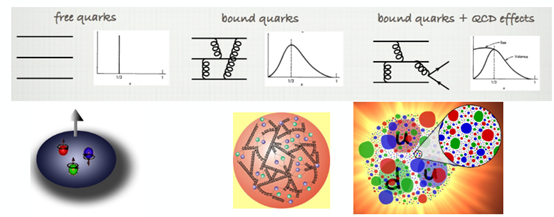
\includegraphics[width = .8\linewidth]{figs/fig_pdf.png}
    \caption{对部分子模型的认识的不断改进。分布函数的横轴是部分子携带总动量的比例，纵轴是概率。}
\end{figure}

部分子分布函数(Parton Distribution Function, PDF)被记作
\n{有时候简写为$f_i(x)$}
\begin{align}
    f_{i/H}(x, \mu_F)
\end{align}
其含义是在给定因子化能标$\mu_F$下，在强子H中找到携带动量分数为x的种类为i的部分子的概率密度。因子化能标区分了强相互作用的高能和低能部分，由于渐近自由效应，高能部分耦合常数$\alpha_s$小，可以用微扰论计算；低能部分是非微扰效应，这部分物理通过PDF体现。
\n{课堂ppt7.2有举例}
在实际的高能物理实验中，以外低能区QCD的复杂，PDF的不确定性（尤其在高x区域）会对实验的分析产生诸多干扰，
伪造“新物理信号”，同时也制约着对标准模型的进一步精确检验。

根据部分子函数的定义，某个部分子所携带动量的期望是：
\begin{align}
    \int_0^1 dx \underbrace{xP}_{\text{部分子携带动量}}f_i(x)
\end{align}

那么期望之和就是强子的总动量：
\begin{align}
    \sum_i \int_0^1 dx \, xPf_i(x) = P
\end{align}
消去常数P可以得到：
\begin{align}
    \sum_i \int_0^1 dx \, xf_i(x) = 1
\end{align}
对于真实的夸克束缚态，夸克的分布实际上由价夸克和海夸克共同构成，通过夸克和反夸克分布的组合，可以表示出价夸克的分布。
\begin{example}[质子和中子]
    对质子(uud)，质子中的u除了价夸克还有胶子辐射所产生的海夸克，而$\bar{u}$只有海夸克部分：
    \begin{align}
        u(x) &= u_{val}(x) + u_{sea}(x) \\
        \bar{u}(x) &= \bar{u}_{val}(x)
    \end{align}
    由此可以组合出价夸克的分布：
    \begin{align}
        u_{val} = u(x)-\bar{u}(x)
    \end{align}
    因为质子含有两个价夸克，所以分布函数满足：
    \begin{align}
        \int_0^1dx[u(x)-\bar{u}(x)] = 2
    \end{align}
    同理有：
    \begin{align}
        \int_0^1dx[d(x)-\bar{d}(x)] = 1
    \end{align}
    做一个同位旋变换就可以得到中子价夸克的结论：
    \begin{align}
        \int_0^1dx[u(x)-\bar{u}(x)] &= 1 \\
        \int_0^1dx[d(x)-\bar{d}(x)] &= 2
    \end{align}
\end{example}